\documentclass[tikz,border=20pt]{standalone}
\usetikzlibrary{calc,arrows.meta,patterns}
\usepackage{xcolor,amsmath}

\definecolor{steelcolor}{HTML}{64748B}
\definecolor{darksteel}{HTML}{1E293B}
\definecolor{rodcolor}{HTML}{CBD5E1}
\definecolor{fluidhigh}{HTML}{EA580C}
\definecolor{fluidlow}{HTML}{0284C7}
\definecolor{sealcolor}{HTML}{0F172A}

\begin{document}
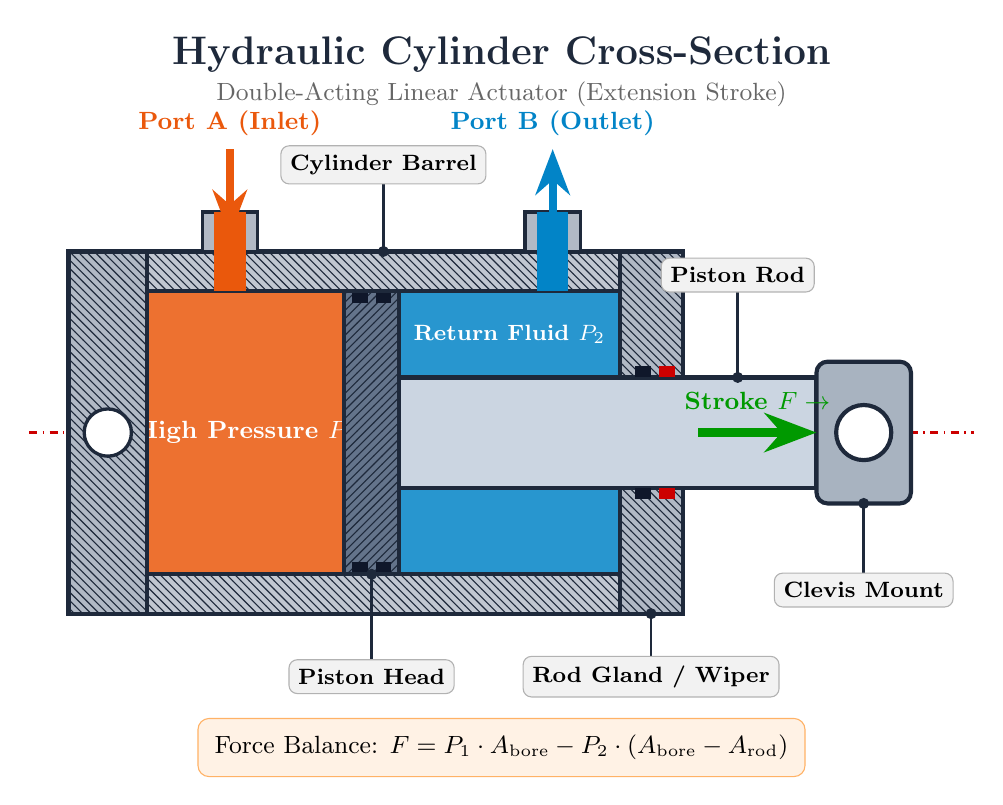
\begin{tikzpicture}[x=1cm, y=1cm, >=Stealth]

  % Title
  \node[font=\bfseries\Large, text=darksteel] at (3.5, 4.8) {Hydraulic Cylinder Cross-Section};
  \node[font=\small, text=gray!80!black] at (3.5, 4.3) {Double-Acting Linear Actuator (Extension Stroke)};

  % Centerline
  \draw[red!80!black, dashdotted, line width=1pt] (-2.5, 0) -- (9.5, 0);

  % High Pressure Fluid (Cap-End Chamber)
  \fill[fluidhigh!85] (-1.0, -1.8) rectangle (1.5, 1.8);
  \node[font=\bfseries\small, text=white] at (0.25, 0) {High Pressure $P_1$};

  % Low Pressure Fluid (Rod-End Chamber)
  \fill[fluidlow!85] (2.2, 0.7) rectangle (5.0, 1.8);
  \fill[fluidlow!85] (2.2, -1.8) rectangle (5.0, -0.7);
  \node[font=\bfseries\footnotesize, text=white] at (3.6, 1.25) {Return Fluid $P_2$};

  % Piston Rod (Chrome Steel)
  \filldraw[fill=rodcolor, draw=darksteel, line width=1.5pt] (2.2, -0.7) rectangle (7.5, 0.7);

  % Rod End Clevis
  \filldraw[fill=rodcolor!80!darksteel, draw=darksteel, line width=1.5pt, rounded corners=4pt]
    (7.5, -0.9) rectangle (8.7, 0.9);
  \filldraw[fill=white, draw=darksteel, line width=1.5pt] (8.1, 0) circle (0.35);

  % Piston Head
  \filldraw[fill=steelcolor, draw=darksteel, line width=1.5pt] (1.5, -1.8) rectangle (2.2, 1.8);
  \fill[pattern=north east lines, pattern color=darksteel] (1.5, -1.8) rectangle (2.2, 1.8);

  % Piston Seals
  \fill[sealcolor] (1.6, 1.65) rectangle (1.8, 1.8);
  \fill[sealcolor] (1.9, 1.65) rectangle (2.1, 1.8);
  \fill[sealcolor] (1.6, -1.8) rectangle (1.8, -1.65);
  \fill[sealcolor] (1.9, -1.8) rectangle (2.1, -1.65);

  % Cylinder Tube Walls (Hatched)
  % Top wall
  \filldraw[fill=steelcolor!40, draw=darksteel, line width=1.5pt] (-1.5, 1.8) rectangle (5.5, 2.3);
  \fill[pattern=north west lines, pattern color=darksteel] (-1.5, 1.8) rectangle (5.5, 2.3);
  % Bottom wall
  \filldraw[fill=steelcolor!40, draw=darksteel, line width=1.5pt] (-1.5, -2.3) rectangle (5.5, -1.8);
  \fill[pattern=north west lines, pattern color=darksteel] (-1.5, -2.3) rectangle (5.5, -1.8);

  % Cap-End Head (Left)
  \filldraw[fill=steelcolor!50, draw=darksteel, line width=1.5pt]
    (-2.0, -2.3) rectangle (-1.0, 2.3);
  \fill[pattern=north west lines, pattern color=darksteel] (-2.0, -2.3) rectangle (-1.0, 2.3);
  \filldraw[fill=white, draw=darksteel, line width=1.2pt] (-1.5, 0) circle (0.3);

  % Rod-End Head / Gland (Right)
  \filldraw[fill=steelcolor!50, draw=darksteel, line width=1.5pt] (5.0, 0.7) rectangle (5.8, 2.3);
  \filldraw[fill=steelcolor!50, draw=darksteel, line width=1.5pt] (5.0, -2.3) rectangle (5.8, -0.7);
  \fill[pattern=north west lines, pattern color=darksteel] (5.0, 0.7) rectangle (5.8, 2.3);
  \fill[pattern=north west lines, pattern color=darksteel] (5.0, -2.3) rectangle (5.8, -0.7);
  % Rod Gland Seals & Wiper
  \fill[sealcolor] (5.2, 0.7) rectangle (5.4, 0.85);
  \fill[red!80!black] (5.5, 0.7) rectangle (5.7, 0.85);
  \fill[sealcolor] (5.2, -0.85) rectangle (5.4, -0.7);
  \fill[red!80!black] (5.5, -0.85) rectangle (5.7, -0.7);

  % Ports & Flow Arrows
  % Port A (Inlet)
  \filldraw[fill=steelcolor!50, draw=darksteel, line width=1.2pt] (-0.3, 2.3) rectangle (0.4, 2.8);
  \fill[fluidhigh] (-0.15, 1.8) rectangle (0.25, 2.8);
  \draw[->, line width=3pt, color=fluidhigh] (0.05, 3.6) -- (0.05, 2.5);
  \node[font=\bfseries\small, text=fluidhigh, above] at (0.05, 3.65) {Port A (Inlet)};

  % Port B (Outlet)
  \filldraw[fill=steelcolor!50, draw=darksteel, line width=1.2pt] (3.8, 2.3) rectangle (4.5, 2.8);
  \fill[fluidlow] (3.95, 1.8) rectangle (4.35, 2.8);
  \draw[<-, line width=3pt, color=fluidlow] (4.15, 3.6) -- (4.15, 2.5);
  \node[font=\bfseries\small, text=fluidlow, above] at (4.15, 3.65) {Port B (Outlet)};

  % Extension Motion Arrow
  \draw[->, line width=3.5pt, color=green!60!black] (6.0, 0) -- (7.5, 0);
  \node[font=\bfseries\small, text=green!60!black, above=2pt] at (6.75, 0.1) {Stroke $F \rightarrow$};

  % Labels with leader lines
  % Cylinder Barrel
  \draw[darksteel, line width=1pt] (2.0, 2.3) -- (2.0, 3.2);
  \fill[darksteel] (2.0, 2.3) circle (2pt);
  \node[draw=gray!60, fill=gray!10, rounded corners=3pt, font=\bfseries\footnotesize] at (2.0, 3.4) {Cylinder Barrel};

  % Piston Head
  \draw[darksteel, line width=1pt] (1.85, -1.8) -- (1.85, -2.9);
  \fill[darksteel] (1.85, -1.8) circle (2pt);
  \node[draw=gray!60, fill=gray!10, rounded corners=3pt, font=\bfseries\footnotesize] at (1.85, -3.1) {Piston Head};

  % Piston Rod
  \draw[darksteel, line width=1pt] (6.5, 0.7) -- (6.5, 1.8);
  \fill[darksteel] (6.5, 0.7) circle (2pt);
  \node[draw=gray!60, fill=gray!10, rounded corners=3pt, font=\bfseries\footnotesize] at (6.5, 2.0) {Piston Rod};

  % Rod Gland & Wiper
  \draw[darksteel, line width=1pt] (5.4, -2.3) -- (5.4, -2.9);
  \fill[darksteel] (5.4, -2.3) circle (2pt);
  \node[draw=gray!60, fill=gray!10, rounded corners=3pt, font=\bfseries\footnotesize] at (5.4, -3.1) {Rod Gland / Wiper};

  % Rod End Clevis
  \draw[darksteel, line width=1pt] (8.1, -0.9) -- (8.1, -1.8);
  \fill[darksteel] (8.1, -0.9) circle (2pt);
  \node[draw=gray!60, fill=gray!10, rounded corners=3pt, font=\bfseries\footnotesize] at (8.1, -2.0) {Clevis Mount};

  % Formula at bottom
  \node[draw=orange!60, fill=orange!10, rounded corners=4pt, font=\small, inner sep=6pt] at (3.5, -4.0) {
    Force Balance: $F = P_1 \cdot A_{\text{bore}} - P_2 \cdot (A_{\text{bore}} - A_{\text{rod}})$
  };

\end{tikzpicture}
\end{document}
